%\RequirePackage[l2tabu, orthodox]{nag}
\documentclass{article}\usepackage[]{graphicx}\usepackage[]{color}
%% maxwidth is the original width if it is less than linewidth
%% otherwise use linewidth (to make sure the graphics do not exceed the margin)
\makeatletter
\def\maxwidth{ %
  \ifdim\Gin@nat@width>\linewidth
    \linewidth
  \else
    \Gin@nat@width
  \fi
}
\makeatother

\definecolor{fgcolor}{rgb}{0.345, 0.345, 0.345}
\newcommand{\hlnum}[1]{\textcolor[rgb]{0.686,0.059,0.569}{#1}}%
\newcommand{\hlstr}[1]{\textcolor[rgb]{0.192,0.494,0.8}{#1}}%
\newcommand{\hlcom}[1]{\textcolor[rgb]{0.678,0.584,0.686}{\textit{#1}}}%
\newcommand{\hlopt}[1]{\textcolor[rgb]{0,0,0}{#1}}%
\newcommand{\hlstd}[1]{\textcolor[rgb]{0.345,0.345,0.345}{#1}}%
\newcommand{\hlkwa}[1]{\textcolor[rgb]{0.161,0.373,0.58}{\textbf{#1}}}%
\newcommand{\hlkwb}[1]{\textcolor[rgb]{0.69,0.353,0.396}{#1}}%
\newcommand{\hlkwc}[1]{\textcolor[rgb]{0.333,0.667,0.333}{#1}}%
\newcommand{\hlkwd}[1]{\textcolor[rgb]{0.737,0.353,0.396}{\textbf{#1}}}%

\usepackage{framed}
\makeatletter
\newenvironment{kframe}{%
 \def\at@end@of@kframe{}%
 \ifinner\ifhmode%
  \def\at@end@of@kframe{\end{minipage}}%
  \begin{minipage}{\columnwidth}%
 \fi\fi%
 \def\FrameCommand##1{\hskip\@totalleftmargin \hskip-\fboxsep
 \colorbox{shadecolor}{##1}\hskip-\fboxsep
     % There is no \\@totalrightmargin, so:
     \hskip-\linewidth \hskip-\@totalleftmargin \hskip\columnwidth}%
 \MakeFramed {\advance\hsize-\width
   \@totalleftmargin\z@ \linewidth\hsize
   \@setminipage}}%
 {\par\unskip\endMakeFramed%
 \at@end@of@kframe}
\makeatother

\definecolor{shadecolor}{rgb}{.97, .97, .97}
\definecolor{messagecolor}{rgb}{0, 0, 0}
\definecolor{warningcolor}{rgb}{1, 0, 1}
\definecolor{errorcolor}{rgb}{1, 0, 0}
\newenvironment{knitrout}{}{} % an empty environment to be redefined in TeX

\usepackage{alltt}

\usepackage{xltxtra} %% For XeTeX font commands
\usepackage[includeheadfoot, margin = 0.5in]{geometry} %% Margins
\usepackage[pageanchor = true]{hyperref}
\usepackage{graphicx} 
\usepackage{sectsty} %% Change format (font) of section headers
\usepackage{tikz}    %% Graphics for banner
%\usepackage[parfill]{parskip} %% Lines between paragraphs, no indentation
\usepackage{booktabs} %% Pretty up the tables
\usepackage[width = .5\textwidth]{caption} %% Width of captions
\usepackage{xcolor}

\usepackage{microtype}
\setlength{\parskip}{1.5ex} %% Space between paragraphs
\setlength{\parindent}{0em} %% No indentation
\clubpenalty = 10000        %% Orphans and widows
\widowpenalty = 10000

% \usepackage[normalem]{ulem} %% For underlines (in the URLs)
% \DeclareUrlCommand{\ulurl}{\uline}

%% Colors
\definecolor{pocDGreen}{HTML}{3D4132}
\definecolor{pocLGreen}{HTML}{9FB78D}
\definecolor{pocDBlue}{HTML}{244356}
\definecolor{pocLBlue}{HTML}{A3DCE6}
\definecolor{pocPurple}{HTML}{A784B4}

%% Fonts
\setmainfont[Ligatures=TeX]{Frutiger LT Std 45 Light}
\allsectionsfont{\fontspec{Archer}}

\usepackage{fancyhdr} %% Header and Footer formatting
\pagestyle{fancy}

%% Hyperlinks, PDF properties
\hypersetup{
    pdftitle = {POC County Report},
    pdfauthor = {Partners for Our Children},
    pdfcreator = {Gregor Passolt},
    pdfproducer = {Gregor Passolt},
    linkbordercolor = cyan,
    %hidelinks,
    unicode = true
}

% \makeatletter
% \DeclareUrlCommand\ULurl@@{%
%   %\def\UrlFont{\ttfamily\color{blue}}%
%   \def\UrlLeft{\uline\bgroup}%
%   \def\UrlRight{\egroup}}
% \def\ULurl@#1{\hyper@linkurl{\ULurl@@{#1}}{#1}}
% \DeclareRobustCommand*\ULurl{\hyper@normalise\ULurl@}
% \makeatother


%%% Header
\renewcommand{\sectionmark}[1]{\markboth{\MakeUppercase{#1}}{\MakeUppercase{#1}}}
\fancyhf{}
\renewcommand{\headrulewidth}{0.5pt}
\renewcommand{\headrule}{\hbox to\headwidth{%
\color{pocDGreen}\leaders\hrule height \headrulewidth\hfill}}
\rhead{\color{pocDGreen} \leftmark}

%%% Footer
\lfoot{\color{pocDGreen} \href{http://www.partnersforourchildren.org}{www.partnersforourchildren.org}}
\rfoot{\color{pocDGreen} \thepage}
\renewcommand{\footrulewidth}{0.5pt}
\renewcommand{\footrule}{\hbox to\headwidth{\color{pocDGreen}\leaders\hrule height \footrulewidth\hfill}}
\IfFileExists{upquote.sty}{\usepackage{upquote}}{}

\begin{document}
\newgeometry{bottom = 0.2in, top = 0.5in, right = 0.5in, left = 0.5in}
\frenchspacing %% Single space after period







\lhead{\color{pocDGreen} Klickitat County Report}
\thispagestyle{empty} %% No header/footer on first page

%\vspace{-2in}

\begin{tikzpicture}[x=1in, y=1in]

    %%    Set up constants
    \def\banX{\textwidth}
    \def\banY{1.9in}
    \def\stripeHeight{0.5in}
    \def\stripeYpos{0.55in} %% From top
    \def\triX{0.25in}
    \def\triY{0.15in}
    \def\logoInsetX{0.7in}
    \def\logoInsetY{18pt}
    
    %% Draw Background Geomety
    \filldraw[pocLGreen] (0, 0) rectangle ++(\banX, \banY);
    \filldraw[pocDGreen] (0, \banY - \stripeYpos) rectangle ++(\banX + \triX, - \stripeHeight);
    \filldraw[fill=pocLGreen, draw=pocDGreen, join=bevel, thick]
        (\banX, \banY - \stripeYpos - \stripeHeight) -- ++(\triX, 0) -- ++(-\triX, -\triY) -- cycle;
    
    %% Above-stripe Text
    \node[pocDBlue, below left = 6pt, align = right] at (\banX, \banY)
        {\textbf{Based on FamLink Data}\\\textbf{Extracted on August 09, 2013}};
    \node at (\logoInsetX, \banY - \logoInsetY)
        {
\includegraphics[height=0.3in]{pocLogoSmall}};
    
    %% Stripe Text
    \node[right = 6pt, white] at (0, \banY - \stripeYpos - \stripeHeight + 16pt)
        {\fontspec{Archer}\Huge{Focus on Klickitat County}};
    
    %% Below Stripe Text
    \node[below right = 6pt, pocDBlue, align = left, text width = \textwidth - 12pt]
        at (0, \banY - \stripeYpos - \stripeHeight) {
         This \emph{Focus on Klickitat County} report is one of a series of automated county reports for Washington State. These quarterly reports mirror the Child Well-Being Data Portal by providing information on three major parts of the child welfare system: Investigations \& Assessments, In-Home Services, and Out-of-Home Care. To access the Data Portal and the latest county reports, visit \href{http://www.partnersforourchildren.org/child-well-being}{www.partnersforourchildren.org/child-well-being}.} ;  
\end{tikzpicture}

\vspace{-18pt}

\section*{Overview}
\vspace{-6pt}
The Department of Social and Health Services (DSHS) divides Washington State into three regions. Klickitat County is in Region~1, along with Adams, Asotin, Benton, Chelan, Columbia, Douglas, Ferry, Franklin, Garfield, Grant, Kittitas, Lincoln, Okanogan, Pend Oreille, Spokane, Stevens, Walla Walla, Whitman and Yakima counties. The following report includes basic graphs and tables for Investigations \& Assessments, In-Home Services and Out-of-Home Care in Klickitat County}.

The Investigations \& Assessments section (page \pageref{p:ia}) and the In-Home Services section (page \pageref{p:ihs}) provide household data on, respectively, the total number of investigations and assessments and in-home service cases since 2009, as well as comparative rates for investigations and assessments and in-home service cases for all Region~1 DCFS (Division of Children \& Family Services) office(s)/office group(s) and for Washington State.
  
The Out-of-Home Care section (page \pageref{p:ooh}) provides total counts and comparative rates for the same time periods, but counts children, not households, and compares across counties rather than offices or office groups. The Out-of-Home Care section also provides basic graphs depicting safety, permanency outcomes and well-being for children in out-of-home care.

\begin{itemize}
\item Safety is measured as the percentage of children who re-entered out-of-home care within two years after already exiting to a permanent placement (i.e., reunification, adoption, and guardianship), with region-level and state-level context. 

\item Permanency outcomes are measured as the percentage of children who entered out-of-home care and experienced one of the following outcomes after two years:  reunification, adoption, guardianship, emancipation, other or still in out-of-home care. 

\item Well-being is measured as the average percent of time children spent in the care of relatives (kinship care) while in out-of-home care during 2009-2010.
\end{itemize}
 
We hope this report serves as a valuable tool for  Klickitat County.

\begin{minipage}{0.6\textwidth}
%\vspace{-1.8in}
\textbf{Data highlights for Klickitat County:}

% latex table generated in R 3.0.1 by xtable 1.7-1 package
% Thu Nov 14 16:38:27 2013
\begin{tabular}{lr}
  \toprule
 \textbf{U.S. Census Bureau (2012)} &  \\ 
  \quad Total Population & 20,699 \\ 
  \quad Percent of Population Under 5 Years & 5.4\% \\ 
  \quad Percent of Population Under 18 Years & 21.7\% \\ 
  \textbf{Child Well-Being Data Portal (April 01, 2013)} &  \\ 
  \quad Number of Open Investigations \& Assessments & 17 \\ 
  \quad Number of Open In-Home Service Cases & 12 \\ 
  \quad Number of Open Out-of-Home Care Cases & 30 \\ 
  \quad Percent of Out-of-Home Care Cases: Children Under 5 Years & 30\% \\ 
   \bottomrule
\end{tabular}



\end{minipage}
\begin{minipage}{0.4\textwidth}

\begin{center}
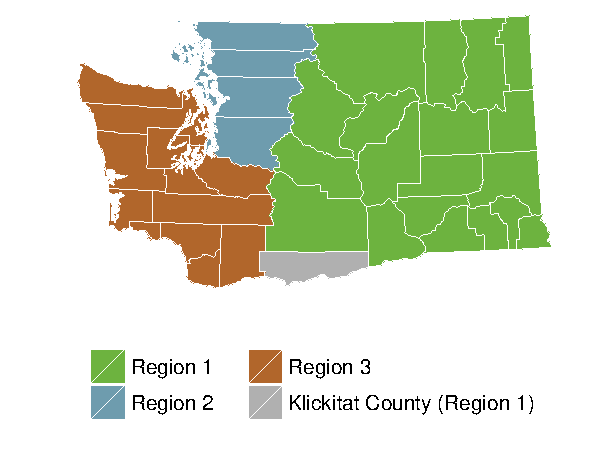
\includegraphics[width=2.7in]{county_maps/Klickitat-b}
\end{center}

\end{minipage}


\newpage
\restoregeometry
\section{\href{http://www.partnersforourchildren.org//child-well-being/visualizations/investigations-assessments/trends}
{Investigations \& Assessments}}
When professionals and community members report suspected instances of child abuse or neglect to the child welfare system, some of the reports are investigated, some are assessed only (e.g., Family Reconciliation Services) and some are screened out because the information reported (if true) does not meet the statutory definition of child abuse or neglect and there is not an immediate need for an assessment or investigation.\\[6pt]
\label{p:ia}

\begin{minipage}{\textwidth}
\subsection{\href{http://www.partnersforourchildren.org//child-well-being/visualizations/investigations-assessments/trends}
{Investigations \& Assessments:} Klickitat County Focus}
The following graph(s) display point-in-time (i.e., first day of the quarter) trends in investigations \& assessments cases for the DCFS office(s)/office group(s) in Klickitat County.  
\begin{knitrout}
\definecolor{shadecolor}{rgb}{0.969, 0.969, 0.969}\color{fgcolor}

{\centering 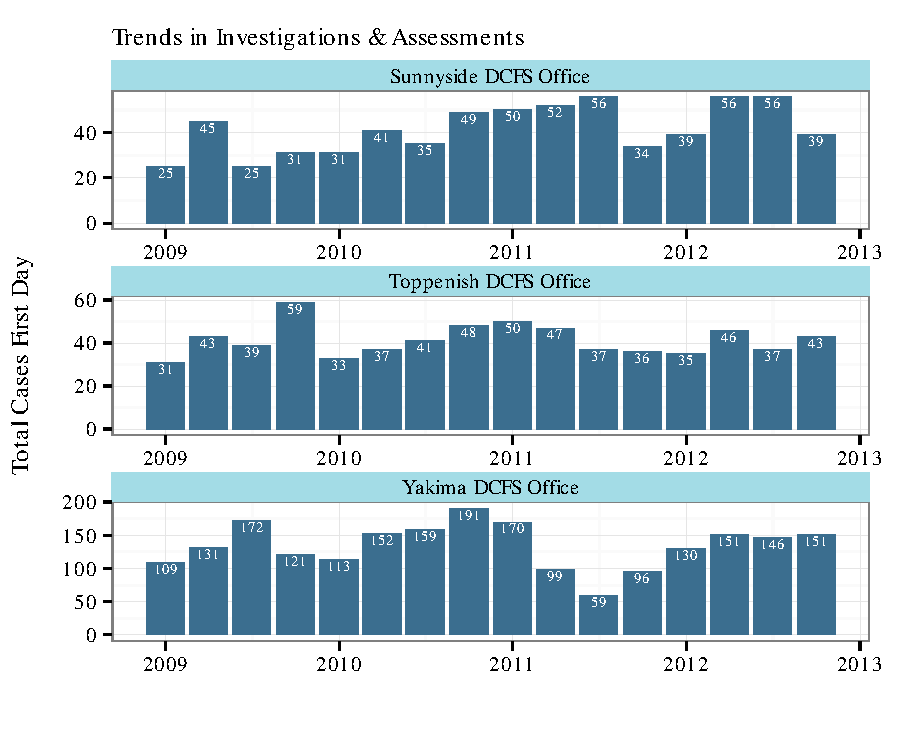
\includegraphics[width=\maxwidth]{figure/ia_focus} 

}



\end{knitrout}

\end{minipage}

\newpage

\subsection{
    \href{http://www.partnersforourchildren.org//child-well-being/visualizations/investigations-assessments/trends}
    {Investigations \& Assessments: Region~1}}
To give context to the Klickitat County offices' trend data, the following plot compares the rate of investigations \& assessments on December 1, 2012 for each Region~1 office/office group and for Washington State.  Rates, rather than counts (or total numbers), are used because they account for the population differences across Washington State counties.
\nopagebreak[3]
\begin{knitrout}
\definecolor{shadecolor}{rgb}{0.969, 0.969, 0.969}\color{fgcolor}

{\centering 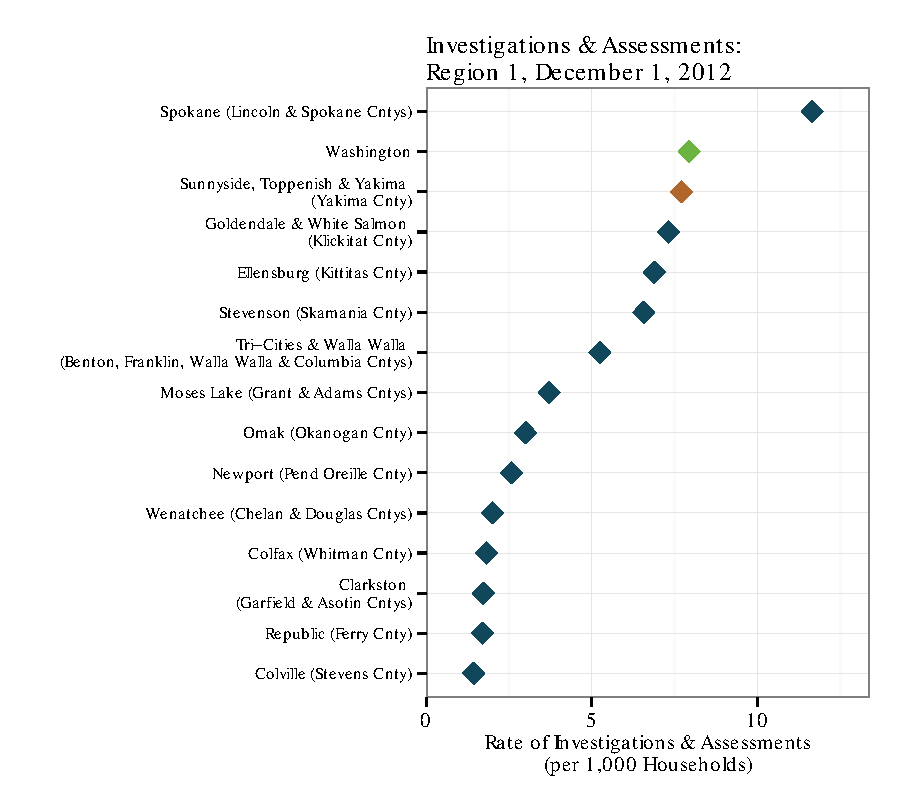
\includegraphics[width=\maxwidth]{figure/ia_context} 

}



\end{knitrout}



%%%%%%%%%%%%%%%%%%%%%%%%%%%%%%%%%%%%%%%%%%%%%%%% ----
\newpage
\section{\href{http://www.partnersforourchildren.org/child-well-being/visualizations/home-services/trends}
    {In-Home Services}
}
When an investigation identifies a threat to a child's safety, case workers will first determine if the child can be kept safely at home through a safety plan. If so, the family and child may be provided with various services that range from concrete support (e.g., food, appliance repair, etc.) to referrals to community services (e.g., drug and alcohol assessments, etc.).\\[6pt]
\label{p:ihs}

\begin{minipage}{\textwidth}
\subsection{\href{http://www.partnersforourchildren.org/child-well-being/visualizations/home-services/trends}
    {In-Home Services: Klickitat County Focus}
}
The following graph(s) display point-in-time (i.e., first day of the quarter) trends in in-home services cases for the DCFS offices in Klickitat County. 
\nopagebreak[3]
\begin{knitrout}
\definecolor{shadecolor}{rgb}{0.969, 0.969, 0.969}\color{fgcolor}

{\centering 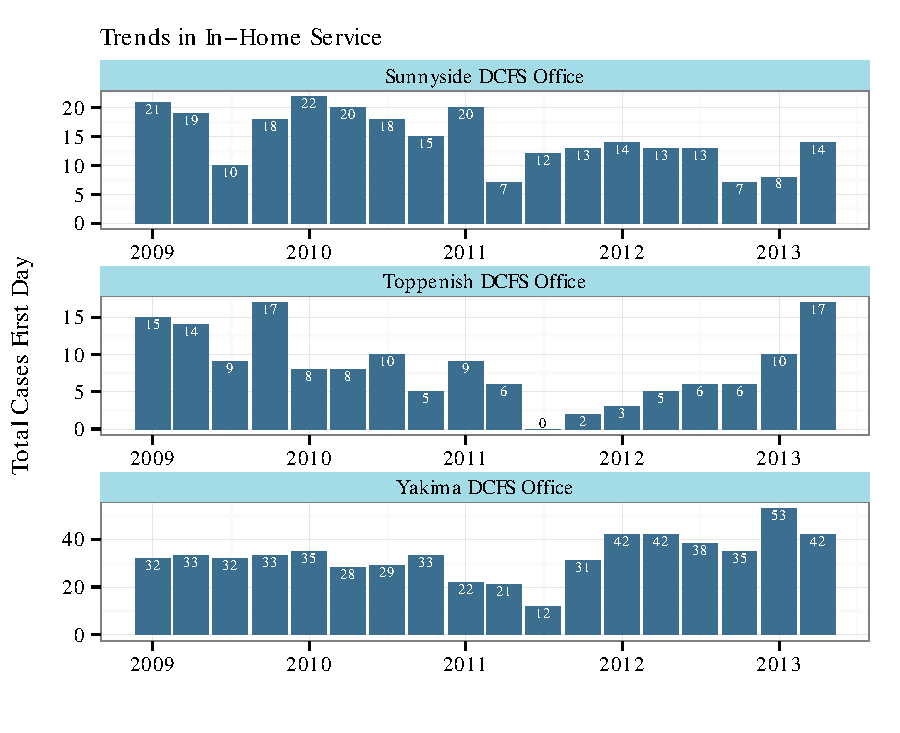
\includegraphics[width=\maxwidth]{figure/ihs_focus} 

}



\end{knitrout}

\end{minipage}

\newpage

\subsection{\href{http://www.partnersforourchildren.org/child-well-being/visualizations/home-services/trends}
    {In-Home Services:} Region~1
}
To give context to the Klickitat County office(s') trend data, the following plot compares the rate of in-home services in quarter 2 of 2013 for each Region~1 office and for Washington State. Rates, rather than a total number, are used because they account for the population differences across Washington State counties.
\nopagebreak[3]
\begin{knitrout}
\definecolor{shadecolor}{rgb}{0.969, 0.969, 0.969}\color{fgcolor}

{\centering 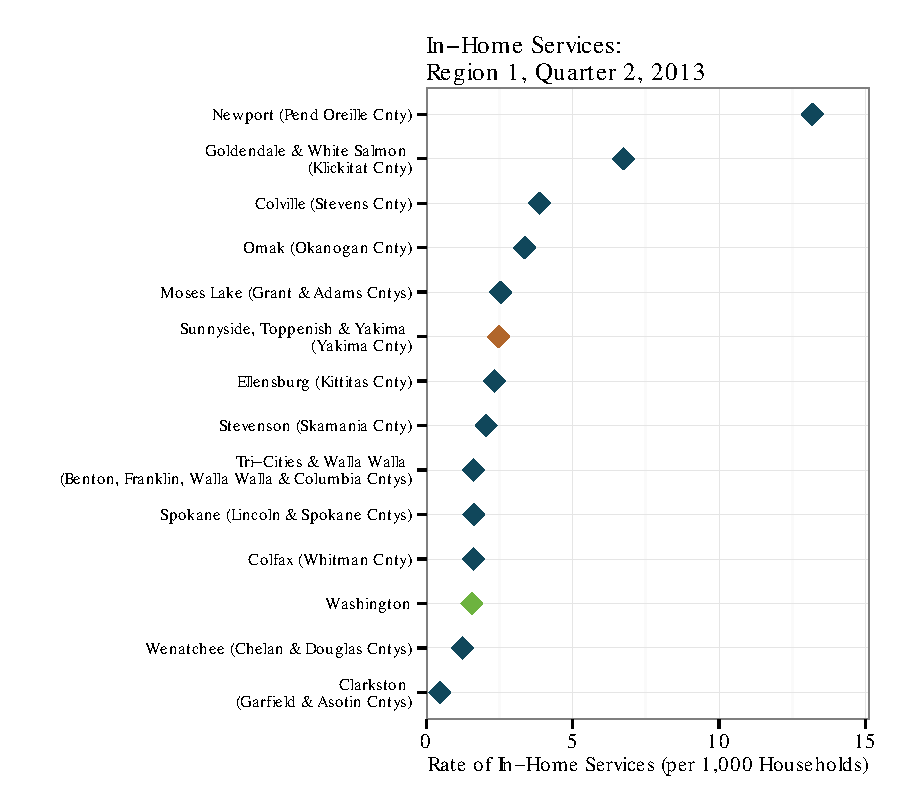
\includegraphics[width=\maxwidth]{figure/ihs_context} 

}



\end{knitrout}


\newpage

\subsection{\href{http://www.partnersforourchildren.org/child-well-being/visualizations/home-services/safety}
    {In-Home Services: Safety}
}
At times, the in-home services provided to families do not, or cannot, adequately address the issues identified during the investigation. Other times, new issues are raised during the course of an in-home services case. Either way, when the case worker decides that it is not possible for the child to remain safely in their home, steps will be taken to place the child in out-of-home care.

The measurements in Table 1 identify placement into out-of-home care among families and their children who have received in-home services. If the in-home services are completed and effective, and/or circumstances become such that the child can remain in-home safely, there should be no need to place the child in out-of-home care. Thus, in general, the lower percentages indicate better outcomes. Note that these percentages are totals; that is, the percentage within two years takes into account the percent from the first year.
\vspace{12pt}
% latex table generated in R 3.0.1 by xtable 1.7-1 package
% Thu Nov 14 16:38:28 2013
\begin{table}[ht]
\centering
\caption{Percent of 2010 In-Home Service Cases Resulting in Out-of-Home Care Placement} 
\begin{tabular}{lrr}
  \toprule
 & Within 1 Year & Within 2 Years \\ 
  \midrule
White Salmon & 11\% & 16\% \\ 
  Washington & 17\% & 20\% \\ 
  Goldendale & 27\% & 30\% \\ 
   \bottomrule
\end{tabular}
\end{table}



%%%%%%%%%%%%%%%%%%%%%%%%%%%%%%%%%%%%%%%%%%%%%%%%% ----
\newpage
\section{\href{http://www.partnersforourchildren.org/child-well-being/visualizations/out-home-care/trends}
    {Out-of-Home Care}
}
When children cannot remain safely in their home, they are placed in out-of-home care. Once a child is removed, the child welfare system works to find a safe and permanent home for the child. Most children ultimately reunify with their parents after all safety concerns have been addressed; however, some children exit to other permanency outcomes (e.g., adoption, guardianship).\\[6pt]

%(Note that the reports for comma_vector(omit_ooh_counties, oxford = FALSE) counties do not contain comparisons in the out-of-home care section due to a small populations, and subsequently, small numbers of out-of-home placements.)
\label{p:ooh}

\begin{minipage}{\textwidth}
\subsection{\href{http://www.partnersforourchildren.org/child-well-being/visualizations/out-home-care/trends}
 {Out-of-Home Care: Klickitat County Focus}
}
The following graphs display point-in-time (i.e., first day of the quarter) trends in out-of-home care cases for
Klickitat County.\\[1pt]
%\nopagebreak[3]
\begin{knitrout}
\definecolor{shadecolor}{rgb}{0.969, 0.969, 0.969}\color{fgcolor}

{\centering 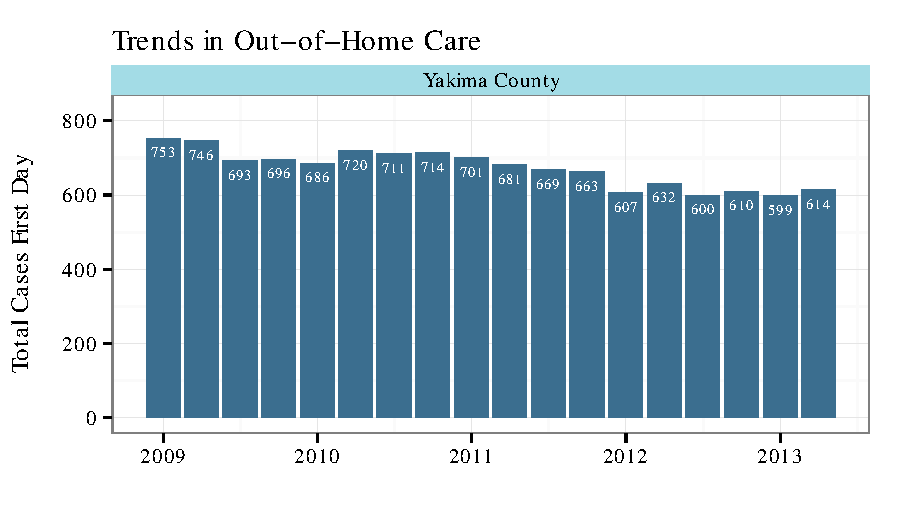
\includegraphics[width=\maxwidth]{figure/ooh_focus} 

}



\end{knitrout}

\end{minipage}
%\newpage

\begin{minipage}{\textwidth}
\subsection{\href{http://www.partnersforourchildren.org/child-well-being/visualizations/out-home-care/trends}
    {Out-of-Home Care: Region~1}
}
To give context to the Klickitat County trend data, the following plot shows the rate of out-of-home care in quarter 2 of 2013 for Region~1 counties and for Washington State. Rates, rather than counts (or total numbers), are used because they account for the population differences across Washington State counties.\\[1pt]
%\nopagebreak[3]
\begin{knitrout}
\definecolor{shadecolor}{rgb}{0.969, 0.969, 0.969}\color{fgcolor}

{\centering 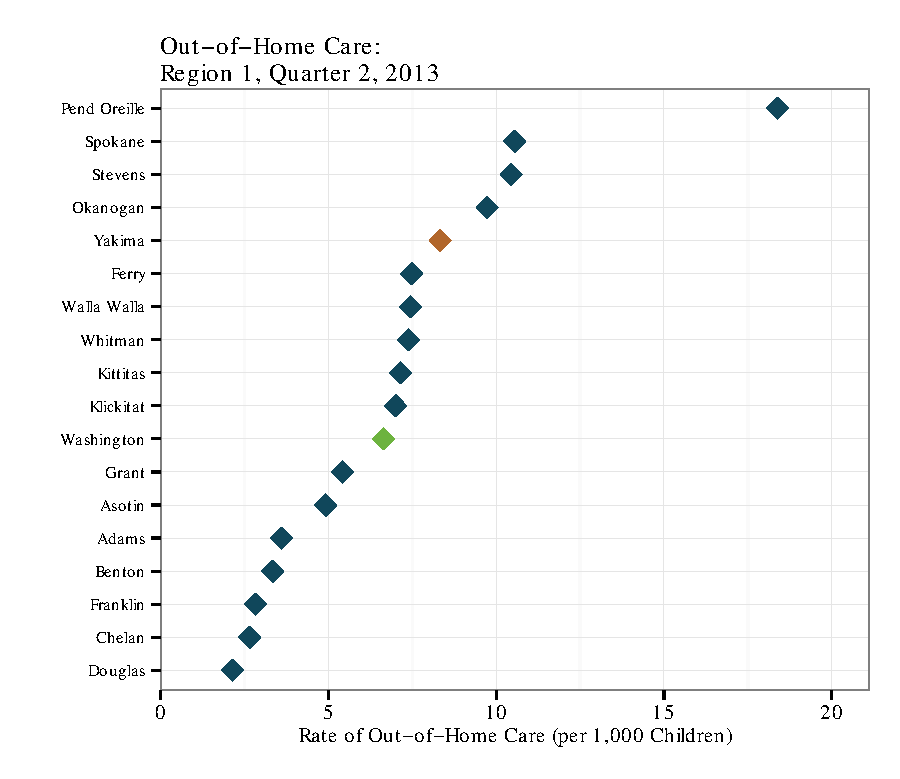
\includegraphics[width=\maxwidth]{figure/ooh_context} 

}



\end{knitrout}

\end{minipage}
\newpage

\subsection{\href{http://www.partnersforourchildren.org/child-well-being/visualizations/out-home-care/safety}
    {Out-of-Home Care: Safety}
}

Sometimes, when children experience a permanency outcome after out-of-home placement (e.g., reunification, guardianship, adoption), safety concerns can resurface. In some circumstances, these safety concerns can be severe enough that the child needs to re-enter out-of-home care.

Table 2 identifies the percentage of children re-entering out-of-home care within two years of exiting to a permanent outcome in 2010, by permanency type, for Region~1 counties, as well as for Washington State overall. The higher percentages of re-entry point to the challenges of providing a safe, permanent outcome for the child.
\vspace{12pt}
\nopagebreak[3]
% latex table generated in R 3.0.1 by xtable 1.7-1 package
% Thu Nov 14 16:38:29 2013
\begin{table}[ht]
\centering
\caption{Percentage of Children Re-Entering Out-of-Home Care within Two Years of Exiting Out-of-Home Care, 2010 Exit Cohort} 
\begin{tabular}{lr}
  \toprule
 & Re-entry from Reunification \\ 
  \midrule
Kittitas & 33.3\% \\ 
  Pend Oreille & 25\% \\ 
  \textbf{Klickitat} & 22.2\% \\ 
  Ferry & 20\% \\ 
  Franklin & 17.2\% \\ 
  Yakima & 14.8\% \\ 
  Spokane & 13.8\% \\ 
  Stevens & 13.6\% \\ 
  \textbf{Washington} & 12.9\% \\ 
  Chelan & 12.5\% \\ 
  Walla Walla & 10.5\% \\ 
  Benton & 7.1\% \\ 
  Okanogan & 6.9\% \\ 
  Grant & 6.1\% \\ 
  Adams & 0\% \\ 
  Douglas & 0\% \\ 
  Whitman & 0\% \\ 
   \bottomrule
\end{tabular}
\end{table}



\newpage

%% Outcomes Chunk
\subsection{\href{http://www.partnersforourchildren.org/child-well-being/visualizations/out-home-care/outcomes}
    {Out-of-Home Care: Outcomes}
}
Under the Adoption and Safe Families Act of 1997 (ASFA), the goal of the child welfare system is to ensure that children are placed in safe and permanent homes as quickly as possible. When it is safe to do so, the child welfare system first seeks to reunify children with their families. If children are unable to be safely reunified, permanency can be achieved through adoption or guardianship. Some children will also exit the system for other reasons, such as emancipation or transfer of custody to different jurisdictions (e.g., Tribal authorities).

The following bar graph shows the percentage of children in the 2010 entry cohort (those who entered at the same time in 2010) achieving each outcome for Klickitat County, Region~1 and Washington State.
\nopagebreak[3]
\begin{knitrout}
\definecolor{shadecolor}{rgb}{0.969, 0.969, 0.969}\color{fgcolor}

{\centering 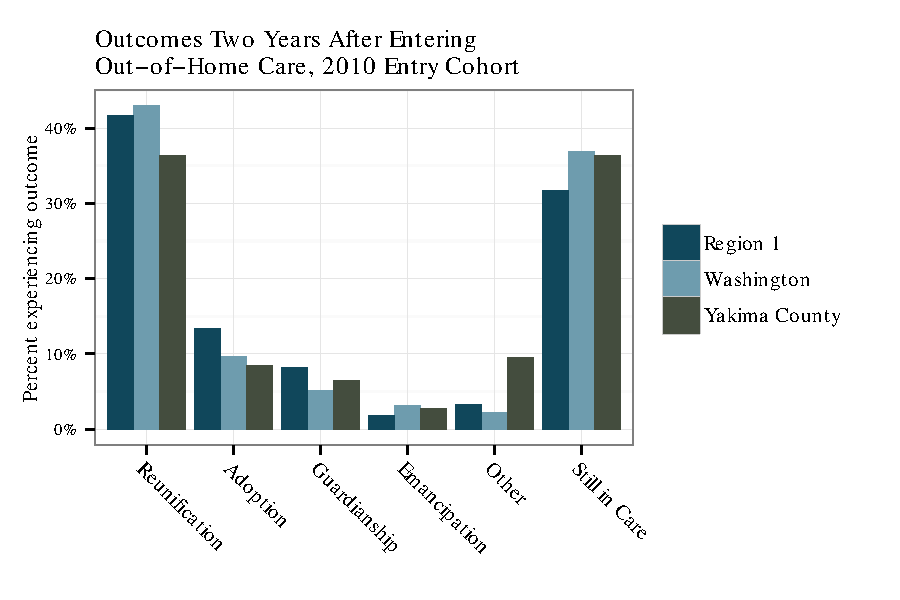
\includegraphics[width=\maxwidth]{figure/ooh_outcomes} 

}



\end{knitrout}


\newpage

%% Well-Being
\subsection{\href{http://www.partnersforourchildren.org/child-well-being/visualizations/out-home-care/well-being}
    {Out-of-Home Care: Well-Being}
}

When placement in out-of-home care is necessary, the physical and psychological needs, as well as the general well-being of the child must be considered. While individual needs vary and well-being is difficult to measure directly, research has shown that placement in kinship care (i.e., a relative's home) can enhance a child's physical and emotional health. Yet, in some cases, the child's best interests necessitate placement in a non-family setting. For example, a child may need specialized services to accomplish a specific therapeutic goal. In such cases, a child may be placed in a non-family setting until those therapeutic goals are met.

Assuming that to some extent kinship care measures child's well-being in an out-of-home setting, the graph below shows the average percent of time that children in out-of-home care spend in kinship care (as opposed to foster care or a non-family setting) for the counties in Region~1. While in out-of-home care, children often stay in different settings. For example, a child can start in a foster home, but then move to kinship care as soon as a willing and able relative is identified. The online Data Portal provides a more detailed look at kinship care, as well as several other measures related to child well-being.

%The online Data Portal provides another view of kinship care. The Portal shows, for instance, that in display_county County on December 1, 2012, 36\% of the children in out-of-home care were in kinship care, while 59\% were in state or private foster care and 5\% were in a non-family placement setting.

\nopagebreak[3]
\begin{knitrout}
\definecolor{shadecolor}{rgb}{0.969, 0.969, 0.969}\color{fgcolor}

{\centering 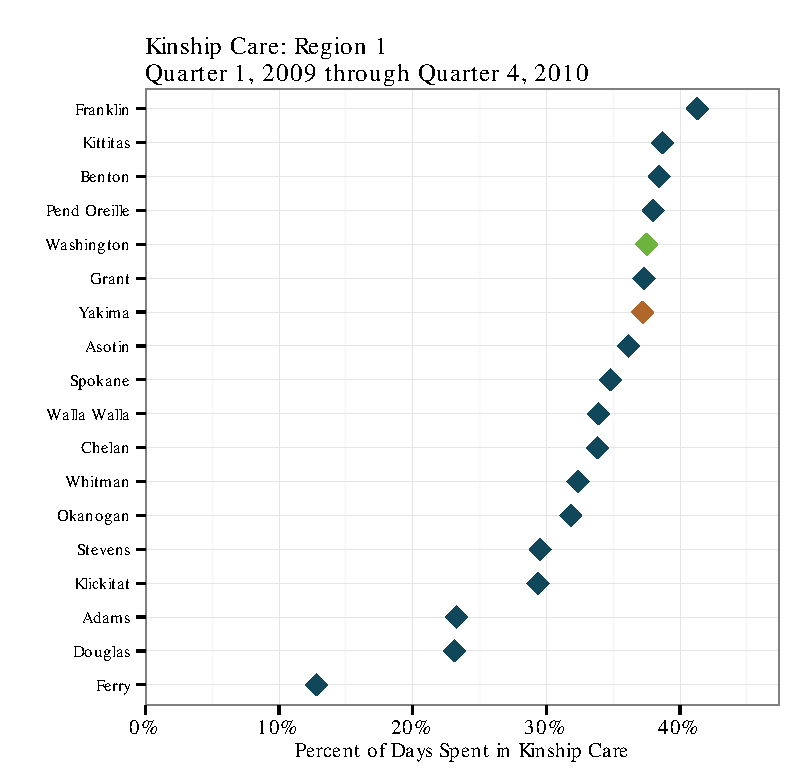
\includegraphics[width=\maxwidth]{figure/ooh_wb} 

}



\end{knitrout}

\vspace{-18pt}

\newpage

\section{Appendix}

The table below provides relevant U.S. Census Bureau data for Klickitat County and for Washington State. 
\nopagebreak[3]
% latex table generated in R 3.0.1 by xtable 1.7-1 package
% Thu Nov 14 16:38:29 2013
\begin{table}[ht]
\centering
\caption{Klickitat County Summary} 
\begin{tabular}{lrr}
  \toprule
 & Klickitat County & Washington \\ 
  \midrule
Total population (2012) & 20,699 & 6,897,012 \\ 
  Percent change in population (2010 to 2012) & 1.9\% & 2.6\% \\ 
  Population under 5 years & 5.4\% & 6.5\% \\ 
  Population under 18 years & 21.7\% & 23.2\% \\ 
  Population: White alone & 93.1\% & 82.0\% \\ 
  Population: Black alone & 0.5\% & 3.8\% \\ 
  Population: American Indian/Alaska Native alone & 2.7\% & 1.8\% \\ 
  Population: Asian alone & 0.8\% & 7.5\% \\ 
  Population: Native Hawaiian/Other Pacific Islander alone & 0.1\% & 0.7\% \\ 
  Population: Multiracial & 2.9\% & 4.3\% \\ 
  Population: Hispanic or Latino Origin & 11.1\% & 11.6\% \\ 
  Population: Not Hispanic, White alone & 83.1\% & 72.1\% \\ 
  Education: High school graduate (age $>$25) & 87.3\% & 89.8\% \\ 
  People below poverty line (all ages) & 18.6\% & 12.5\% \\ 
  Population per square mile & 10.9 & 101.2 \\ 
   \bottomrule
\end{tabular}
\end{table}



U.S. Census data is retrieved from the most recent State and County Quickfacts (\href{http://quickfacts.census.gov/qfd/states/53000.html}{http://quickfacts.census.gov/qfd/states/53000.html}).\\

\textbf{Note:} In this report, data are presented using ``unduplicated counts,'' meaning each household with at least one open investigation or one open in-home service case on the first day of the quarter was counted. Unduplicated counts for out-of-home care cases means each child in out-of-home care on the first day of the quarter was counted (see \href{http://http://www.partnersforourchildren.org/publications/using-different-count-types-data-portal}{Technical Bulletin: Interpreting the Type of Count Filter} for more information).  
\end{document}

